\chapter{Marco Teórico}

Antes de avanzar en los capítulos de este documento, es de vital importancia aclarar los conceptos utilizados de modo que exista una base de conocimiento que permita la total comprensión de los temas tratados.

\section{StarCraft II}

No todos los videojuegos son iguales y StarCraft II no es una excepción, por lo que detallar algunos de sus términos es de gran utilidad para la comprensión del documento.

\subsection{Características generales}

Similar a otros juegos del género de estrategia en tiempo real, StarCraft II consiste principalmente de construir un \textbf{ejército} al gestionar los distintos recursos no renovables que existen en el campo de batalla (o \textbf{mapa} de ahora en adelante) con la finalidad de vencer al ejército rival. Todo esto sin turnos establecidos como en otros tipos de juegos de estrategia, pues al tratarse de un juego en tiempo real cada segundo desaprovechado solamente beneficia al oponente y su creciente ejército. Conociendo ya este objetivo de vencer al ejército del oponente, se puede decir que la victoria en una partida se obtiene al derrotar a todas las fuerzas que componen a dicho ejército o cuando el oponente, por voluntad propia, decide rendirse antes de que caiga su ejército.

Antes de iniciar una partida de StarCraft II, cada jugador debe escoger una de las tres \textbf{razas} existentes en el videojuego, las cuales poseen elementos muy distintos entre ellas, pero que se rigen bajo las mismas reglas. Como el documento se basa en la raza Terran, las definiciones y los ejemplos presentados en los capítulos que proceden se enfocan en la raza Terran, aún cuando muchos de estos términos aplican también a las razas Protoss y Zerg.

Una vez iniciado el juego, cada jugador recibe los elementos básicos para comenzar la creación de su ejército: doce trabajadores (\textit{SCV} en el caso de la raza Terran) y un edificio principal (\textit{Command Center} para la raza Terran). A partir de aquí, el jugador tiene libre albedrío para construir su ejército o atacar a las fuerzas enemigas.

\subsection{Árbol de tecnologías}

Si bien existen distintos tipos de entidades que componen la milicia de un jugador, el videojuego los divide en tres categorías que engloban las características de estos: unidades, edificios y mejoras. Aunque existen fuertes similitudes entre todas estas categorías, como el hecho de que todos poseen \textbf{requisitos} de alguna índole, sus funciones principales son muy distintas entre sí.

Las \textbf{unidades} son todas aquellas entidades que son producidas por algún edificio. Su papel consiste, principalmente, en ser la fuerza de ataque de un ejército al movilizarse por el mapa, aunque sus funciones no se limitan sólo a atacar, pues también existen unidades conocidas como \textbf{trabajadores} (que en el caso de la raza Terran reciben el nombre de \textit{SCV} o \textit{Space Construction Vehicles}) los cuales se encargan de la recolección de recursos y también de la construcción de edificios. Al tratarse de entidades que pueden participar en combate, existen \textbf{estadísticas} (como salud, armadura o ataque) asignadas a cada tipo de unidad.

Los \textbf{edificios} son estructuras construidas por los trabajadores o evolucionadas de otros edificios, que se encuentran generalmente fijados a una posición en el mapa (escogida por el jugador al momento de su creación). Su función primordial consiste en la creación de las distintas unidades, aunque su utilidad no se detiene ahí, ya que algunos edificios también poseen características defensivas, otros permiten la investigación de mejoras e incluso uno que aumenta la cantidad de \textbf{suministros} (necesarios para la producción de unidades). De igual manera que las unidades, los edificios poseen estadísticas ya que pueden ser destruidos, aunque sólo algunos tienen estadísticas de ataque.

Tal como indica su nombre, las \textbf{mejoras} ofrecen distintos tipos de beneficios al resto de entidades, los cuales van desde aumentos en sus estadísticas (como aumentos en el ataque o la defensa) hasta el desbloqueo de \textbf{habilidades} que sólo pueden usar unidades o edificios específicos. A diferencia de las unidades o los edificios, las mejoras sólo permiten la creación de una de cada mejora por partida. Como ejemplo se tiene que sólo se puede construir un \textit{Infantry Weapons Level 1} (mejora Terran) a la vez que puedes tener 10 o 15 \textit{Marines} (unidad Terran).

A causa de que a lo largo de este documento se suelen englobar estas tres categorías, es que a partir de ahora se referirá a las unidades, a los edificios y a las mejoras (tanto en conjunto como individualmente) cómo \textbf{entidades}.

Entendiendo las tres categorías de entidades, es que ahora se puede definir al \textbf{árbol de tecnologías} como las relaciones que tiene cada entidad con respecto al resto, el cual nos muestra los \textbf{requisitos} para desbloquear cada entidad (entidades que se necesitan antes de que la unidad en cuestión pueda ser creada) y su \textbf{entidad de creación} (entidad que se encarga de la creación de la entidad en cuestión, que en algunas ocasiones se transforma en esta entidad) tal como se puede observar en la {\ref{fig:2}}.

\begin{figure}[H]
	\centering
	\captionsetup{justification=centering}
	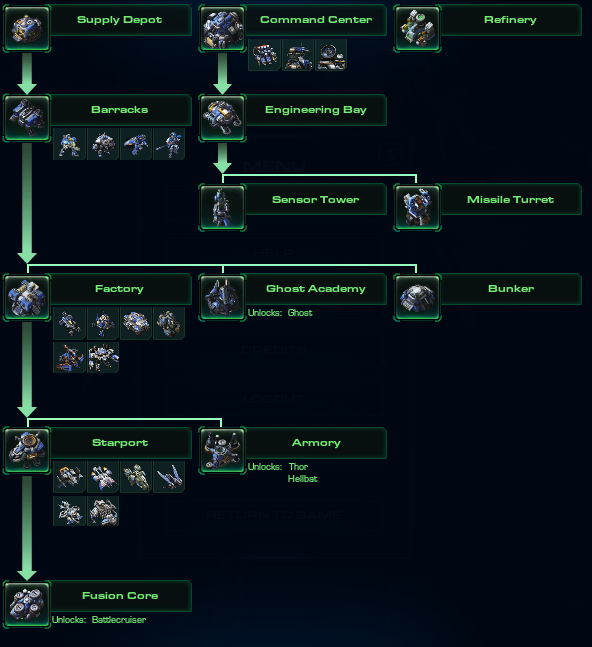
\includegraphics[keepaspectratio]{images/2.png}
	\captionimg{Árbol de tecnologías}{(Blizzard Entertainment, 2021)}
	\label{fig:2}
\end{figure}

\subsection{Economía}

Cómo todo en la vida, cualquiera de las fuerzas previamente mencionadas viene con un costo que varía según la utilidad de cada una. Existen dos tipos de \textbf{recursos} no renovables (minerales y gas vespeno), representados en el juego por números enteros, que son obtenidos por medio de los trabajadores y que son sustraídos cada vez que la creación de una entidad lo requiera y en las cantidades que se especifique. Es importante aclarar que estos recursos no pueden ser menores que cero en ningún caso.

Los \textbf{minerales} son la fuente principal de recursos en StarCraft II, pues todas las entidades lo requieren para comenzar su proceso de creación. Estos minerales son extraídos directamente de los campos de minerales que se encuentran en el mapa por los \textit{SCV}, para luego ser llevados a un \textit{Command Center} (o cualquier edificio que evolucione de este) en donde pasan a ser contabilizados en la cantidad de minerales obtenidos.

\begin{figure}[H]
	\centering
	\captionsetup{justification=centering}
	
\includegraphics[keepaspectratio]{images/minerals.png}
	\captionimg{Minerales}{(Blizzard Entertainment, 2021)}
	\label{fig:3}
\end{figure}

Al comienzo de la partida, la base del jugador inicia en la cercanía de cuatro campos de minerales grandes (que otorgan un máximo de 1800 minerales cada uno) y cuatro pequeños (900 minerales cada uno) resultando en un máximo total de 10800 minerales por base. Si bien estos recursos son limitados y no renovables, el jugador puede encontrar nuevos campos de minerales a lo largo del mapa en las mismas cantidades que los que aparecen en la base inicial, para los cuales es recomendable construir un nuevo \textit{Command Center} que permita depositar el mineral de forma más expedita.

A la hora de extraer los minerales, un \textit{SCV} tarda 1.99 segundos desde que comienza hasta que obtiene los 5 de mineral que puede cargar para, luego, esperar por, aproximadamente, 0.3571 segundos antes de devolverse al \textit{Command Center} para depositarlos y generar un \textbf{ingreso} de 5 minerales. Debido a que sólo se admite un trabajador por mineral a la vez, es que ocurre un fenómeno denominado \textbf{saturación} en dónde se busca maximizar el ingreso al minimizar la aparición de colas de trabajadores que intentan acceder a un mismo mineral, pues cada segundo a la espera es un segundo perdido. Básicamente, hasta dos \textit{SCV} pueden encargarse de un mismo mineral sin que tengan que esperar a que el otro finalice (ambos tienen una \textbf{eficiencia} del 100\% en cuanto al ingreso que obtienen), pero, al ser el objetivo principal el de recolectar la mayor cantidad posible de mineral en el tiempo, es que se ha calculado que el óptimo es de 3 trabajadores por mineral (demostrado visualmente en el juego con un total de 24 \textit{SCV} por base), donde el tercer trabajador recibe menos minerales por unidad de tiempo, pero se maximiza el ingreso total por cada mineral. Con esto en mente, los cálculos realizados por un usuario de la comunidad de StarCraft II (PiousFlea, 2010) arrojan un total aproximado de 102 minerales por minuto al contar con 3 trabajadores por mineral.

Un caso particular ocurre con la unidad \textit{MULE} que puede obtener 4 veces los minerales que un \textit{SCV} y no satura los minerales (ignora las colas), pero con la diferencia de que es una unidad temporal que desaparece pasados 65 segundos desde su creación, cuyo único requisito es la utilización de energía desde un \textit{Orbital Command}. La \textbf{energía} es un recurso renovable que es característico sólo a algunas entidades como el \textit{Orbital Command}, pero que sólo es utilizado para la creación instantánea de otras entidades por este último en la creación de un \textit{MULE} o la investigación de \textit{Extra Supplies}, mientras que el resto de las entidades que poseen energía, la gastan en el uso de distintas habilidades. Las entidades suelen comenzar con 50 de energía, la cual aumenta en 0.7875 cada segundo hasta un máximo de 200, siendo este recurso independiente para cada instancia de entidad.

Por otro lado, el \textbf{gas vespeno} es un recurso más limitado (sólo dos \textbf{géiseres} de gas por base) que no necesitan todas las unidades, pero que no deja de ser vital para construir entidades más poderosas que las que requieren solamente del mineral. A diferencia del anterior que puede ser extraído directamente de los géiseres de gas, el gas vespeno necesita de la creación de un \textit{Refinery} para que los \textit{SCV} puedan extraer el recurso y llevarlo al \textit{Command Center} para que se agregue a la cantidad de gas total.

\begin{figure}[H]
	\centering
	\captionsetup{justification=centering}
	
\includegraphics[keepaspectratio]{images/gas.png}
	\captionimg{Géiseres de gas vespeno}{(Blizzard Entertainment, 2021)}
	\label{fig:4}
\end{figure}

Para la extracción de gas, un \textit{SCV} tarda 1.415 segundos en la extracción del recurso desde el \textit{Refinery} y se dirige inmediatamente a la base a depositar un ingreso igual a los 4 de gas vespeno. Al igual que los minerales, el gas vespeno alcanza la saturación a los 3 trabajadores (total de 6 por base), dando un total de 114 de gas por minuto.

Catalogado también como recurso, aunque con un comportamiento muy distinto al de los dos anteriormente vistos, se tiene el suministro, que es un requisito exclusivo de las unidades. El \textbf{suministro} es un valor entero que limita la cantidad de unidades que se pueden poseer, pues cada una tiene un valor definido que va desde 1 hasta 6 y que se suma para obtener la cantidad actual de suministro del ejército de cada jugador y que debe ser menor que el \textbf{suministro total} que ofrecen algunos edificios. El suministro total es simplemente la suma de 15 veces la cantidad de \textit{Command Centers} o edificios que evolucionen de este más 8 veces la cantidad de \textit{Supply Depots} (edificio) o 16 veces si es que el \textit{Supply Depot} tiene un \textit{Extra Supplies} vinculado. En el caso de agregar una unidad a la cola de creación de cualquier edificio y que el valor de los suministros actuales (contando a la unidad que se desea construir) exceda el de los suministros totales, esta unidad no podrá ser puesta en cola hasta que los suministros totales aumenten.

\subsection{Velocidad de juego}

Al tratarse de un juego en tiempo real es normal que las acciones sean medidas en segundos o fracciones de estos, pero dado que StarCraft II introduce la función de cambiar la \textbf{velocidad de juego} es que se debe explicar en que consiste para poner todo bajo el mismo contexto. El videojuego ofrece cinco velocidades de juego que pueden ser escogidas al crear una partida personalizada o es establecida en la velocidad más alta en caso de que se trate de una partida con emparejamiento automático (partidas clasificatorias). Los \textbf{factores de velocidad} de cada velocidad de juego, cuyos valores están indicados en la tabla {\ref{tab:1}}, dividen los segundos reales para calcular el tiempo de los elementos del juego que lo requieran.

\begin{table}[H]
\centering
\def\arraystretch{1.8}
\captionsetup{justification=centering}
\caption{Tabla de velocidades de juego}
\label{tab:1}
\resizebox{\textwidth}{!}{%
\begin{tabular}{|c|c|c|}
\hline
\textbf{Velocidad de Juego} & \textbf{Factor de Velocidad} & \textbf{Segundos de Tiempo Real en 1 Minuto de Juego \textit{Normal}} \\
\hline
Slower & 0.6 & 100 \\ \hline
Slow & 0.8 & 75 \\ \hline
Normal & 1.0 & 60 \\ \hline
Fast & 1.2 & 50 \\ \hline
Faster & 1.4 & 42.86 \\ \hline
\end{tabular}%
}
\caption*{\textbf{Fuente}: Elaboración Propia, 2021}
\end{table}

Para ejemplificar lo anterior, se puede decir que un \textit{Supply Depot}, que tarda 30 segundos reales en crearse a una velocidad de juego \textit{normal}, tardará aproximadamente 21 segundos reales (21.423, pero el juego aproxima estos valores a un número entero) al utilizar la velocidad de juego \textit{faster}.

La lectura de este documento debe ser abordada teniendo en cuenta la velocidad de juego \textit{faster} como la velocidad por defecto, que es la que se utiliza en partidas clasificatorias y en torneos oficiales. Con esto presente, es importante aclarar que los valores en tiempo mencionados en las secciones anteriores, así como en las secciones por venir, son los que se obtienen en el juego al usar esta velocidad de juego \textit{faster}, lo cual afecta principalmente a los tiempos que tardan en crearse las entidades y los tiempos en que los trabajadores recolectan recursos.

\subsection{Órdenes de construcción}

Si bien ya han sido mencionados a lo largo del documento, aún no se establece una definición concreta sobre los órdenes de construcción.

Cada vez que un jugador comienza la producción de una unidad, la construcción de un edificio o la investigación de una mejora se dice que el jugador está realizando una \textbf{acción}, la cual ocurre en un tiempo determinado contado a partir del inicio de la partida. Al reunir estas acciones en una secuencia, ordenada según sus marcas de tiempo respectivas, se tiene lo que se denomina \textbf{orden de construcción} (conocido en inglés como \textit{Build Order}), el cual se muestra al final de cada partida. Este término no es usado sólamente para referirse a las secuencias que aparecen después de una partida, sino que también se habla de estas series de acciones para referirse a órdenes de construcción "ideales", los cuales tienen las mismas características, pero son secuencias ideales que un jugador debe seguir para alcanzar una o varias entidades deseadas.

Es habitual en la comunidad de StarCraft II que los jugadores compartan estos órdenes de construcción con la finalidad de que sean evaluados por otros jugadores, por lo que no es extraño que se observen distintos formatos a la hora de presentarlos, algunos con elementos extra que facilitan la visualización y comprensión de los mismos. A modo de ejemplo de esto, se puede observar en la figura {\ref{fig:1}} como un orden de construcción puede tener otros valores además de los dos principales (el tiempo y la entidad construida) como la cantidad de suministros máximos y la cantidad de suministros actuales para entregar mayor contexto de la partida, así cómo también existen formatos que utilizan esto último para no incluir la creación de trabajadores con el fin de acortar el tamaño total del orden de construcción.

\begin{figure}[H]
	\centering
	\captionsetup{justification=centering}
	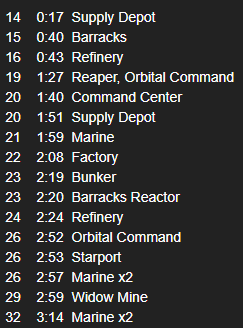
\includegraphics[keepaspectratio]{images/1.png}
	\captionimg{Parte de un orden de construcción}{(Spawning Tool, 2021)}
	\label{fig:1}
\end{figure}

\section{StarCraft II como problema de optimización}

El \textbf{problema de planificación de proyecto con recursos limitados} (Artigues, 2008), mejor conocido como RCPSP (\textit{Resource Constrained Project Scheduling Problem}), es un problema de optimización combinatorial que involucra el manejo de los distintos requisitos obligatorios asociados a un problema con el fin de obtener una \textbf{planificación} de duración mínima, siempre respetando las relaciones de precedencia existentes y la disponibilidad de los recursos.

Un RCPSP se considera como tal al poseer \textbf{actividades} que componen el problema, cuyo inicio se representa como una marca de tiempo denominada \textit{\textbf{schedule}}, y que pueden ser vistas como hitos dentro de esta, además de que cada una de estas actividades tiene una \textbf{duración} asignada y \textbf{relaciones de precedencia} que obligan a que una actividad $A_{j}$ necesite de una previa actividad $A_{i}$ antes de comenzar. Estas actividades no solo requieren de otras, sino que, también, se ven afectadas por la \textbf{demanda} de \textbf{recursos renovables} con distinta \textbf{disponibilidad}.

Con esto en mente y luego de contrastar el RCPSP con las características del videojuego, quedan en evidencia las similitudes entre ambos problemas, permitiendo declarar el \textit{problema de los órdenes de construcción} como un problema de planificación de proyecto con recursos limitados. Las \textit{actividades} describen a la perfección a la creación de las distintas entidades que componen un orden de construcción, pues cada una de ellas tiene una \textit{duración} particular desde que inicia su creación y \textit{relaciones de precedencia} en las distintas entidades requisito que cada una posee. Y esto no es todo, pues la creación de entidades también \textit{demanda} suministros, además de los \textit{recursos renovables}, mineral y gas vespeno cuyas \textit{disponibilidades} varían según la cantidad de trabajadores y su ubicación en el mapa. Para ejemplificar esto, se usa a la unidad \textit{Ghost}, cuya creación tarda 29 segundos en un tiempo de juego \textit{faster}, que debe ser construida en el edificio \textit{Barracks}, pero también requiere que el edificio \textit{Ghost Academy} haya sido creado antes de poder iniciar su propia creación, la cual necesita 150 de mineral, 125 de gas vespeno y al menos 2 de suministro disponible.

\section{Metaheurísticas}

Aún sin garantía de encontrar el óptimo global, las metaheurísticas permiten atacar problemas de optimización para obtener soluciones satisfactorias en un tiempo razonable (Young, 2009). La palabra \textbf{heurística} viene del griego \textit{heuriskein} que se refiere al "arte de descubrir nuevas estrategias o reglas para resolver problemas", mientras que el \textit{meta} en metaheurística significa "metodología de nivel superior", por lo que las \textbf{metaheurísticas} se definen como metodologías generales de nivel superior que pueden ser usadas como estrategias guía al diseñar heurísticas adyacentes para resolver problemas de optimización específicos.

Existen diversos métodos para clasificar a las metaheurísticas. Un ejemplo de esto es clasificarlas según su inspiración al separar aquellas metaheurísticas inspiradas en la naturaleza de las no inspiradas en la naturaleza, pero en esta oportunidad usará la clasificación según el tipo de solución sobre la que trabaja el algoritmo: algoritmos basados en población y algoritmos basados en solución única.

\subsection{Algoritmos de población}

Los \textbf{algoritmos de población} son un tipo de metaheurísticas, los cuales pueden ser vistos como una evolución de una población (conjunto) de soluciones que, de forma iterativa, se va integrando con la población de soluciones actual por medio del uso de procedimientos de selección, permitiendo una mejor diversificación en el espacio de búsqueda, de forma complementaria a los algoritmos de solución única. Ejemplos de este tipo de metaheurística se pueden ver en \textit{algoritmos evolucionarios}, \textit{scatter search} y \textit{algoritmos de estimación de distribución}.

\subsection{Algoritmos de solución única}

Aquellas metaheurísticas que, a diferencia de los algoritmos de población, buscan mejorar sólo una solución son denominadas como \textbf{algoritmos de solución única}, pues recorren el espacio de búsqueda saltando de una solución actual a otra de forma iterativa con la intención de acercarse al óptimo global al intensificar la búsqueda en regiones locales. Algunos ejemplos de este tipo de metaheurísticas son \textit{Simulated Annealing}, \textit{Local Search} y \textit{Tabu Search}.

Entre los conceptos comunes para las metaheurísticas con algoritmos de solución única se encuentran los \textbf{vecindarios}, estructuras de soluciones asociadas a una solución particular, o las \textbf{soluciones iniciales}, que son utilizadas para comenzar cada algoritmo y que puede ser obtenida de manera aleatoria o con un acercamiento \textit{greedy}.

\subsection{Simulated Annealing}

La solución propuesta consta del modelo bajo un enfoque metaheurístico, que incluye un algoritmo capaz de encontrar buenos órdenes de construcción para llegar a una unidad, una tecnología o una estructura de la raza Terran en StarCraft II. Esto, según se especifique antes de la ejecución del algoritmo y optimizando el criterio del tiempo de partida para llegar a dicha unidad, estructura o tecnología. La metaheurística a utilizar será \textbf{\textit{Simulated Annealing}} (SA a partir de ahora), la cual es una metaheurística de algoritmo de solución única que busca imitar el proceso de recocido de algunos metales para obtener el material en un estado más puro o, en este caso, acercarse al óptimo. Si se ve como algoritmo, SA tiene como objetivo escapar del óptimo local de forma en que las generaciones no queden atrapadas en una solución particular. Comenzando con una solución inicial, SA genera un vecino en cada iteración, el cual es seleccionado siempre que mejore la función de costo, pero que en caso de que no mejore esta función, tiene una probabilidad de ser seleccionado según la temperatura (parámetro de control definido acorde al problema) y la diferencia entre los resultados de la función objetivo de las soluciones en comparación. \newline

\begin{algorithm}[H]
    \SetKwData{Left}{left}
    \SetKwData{This}{this}
    \SetKwData{Up}{up}
    \SetKwFunction{Union}{Union}
    \SetKwFunction{FindCompress}{FindCompress}
    \SetKwInOut{Input}{input}
    \SetKwInOut{Output}{output}

    \KwIn{Calendario de enfriamiento}
    \caption{Simulated Annealing}\label{alg:sa}
    
    $s \gets s_{0}$; \tcc{Generación de la solución inicial}\
    $T \gets T_{0}$; \tcc{Temperatura inicial}
    
    \While{Criterio de detención no satisfecho}{
        \While{Condición de equilibrio no satisfecha}{
            Se genera un vecino aleatorio $s'$\;
            $\Delta E \gets f(s') - f(s)$\;
            \If{$\Delta E \leq 0$}{
                $s \gets s'$; \tcc{Acepta la solución vecina}
            }
            \Else{
                $s \gets s'$;\tcc{Acepta s' con una probabilidad $e^\frac{-\Delta E}{T}$}
            }
        }
        $T \gets g(T);$ \tcc{Actualización de temperatura}
    }
    \KwOut{Mejor solución encontrada} 
\end{algorithm}

\section{I-Race}

Aún antes de ejecutar el algoritmo para optimizar las soluciones, es importante optimizar los parámetros que SA recibe con la finalidad de obtener los mejores resultados posibles; a este proceso recién descrito se le denomina \textbf{parametrización}. Ahora, utilizando el paquete de R \textit{\textbf{i-race}} es posible conseguir esta parametrización de forma automática al entregarle conjuntos o rangos de posibles parámetros para que el algoritmo de \textit{i-race} ejecute reiteradamente el algoritmo cuyos parámetros se busca optimizar, que en este caso se trata de SA aplicado al problema de los órdenes de construcción, hasta que se cumpla el \textbf{presupuesto} o número de ejecuciones previamente ajustado. Finalmente se obtendrá una tabla con los mejores parámetros posibles de entre los entregados, el cual debe ser utilizado en las futuras ejecuciones del algoritmo SA.